\section{Messergebnisse und Auswertung}

\subsection{Energieeichung des MCAs}
\begin{figure}[H]
\begin{center}
  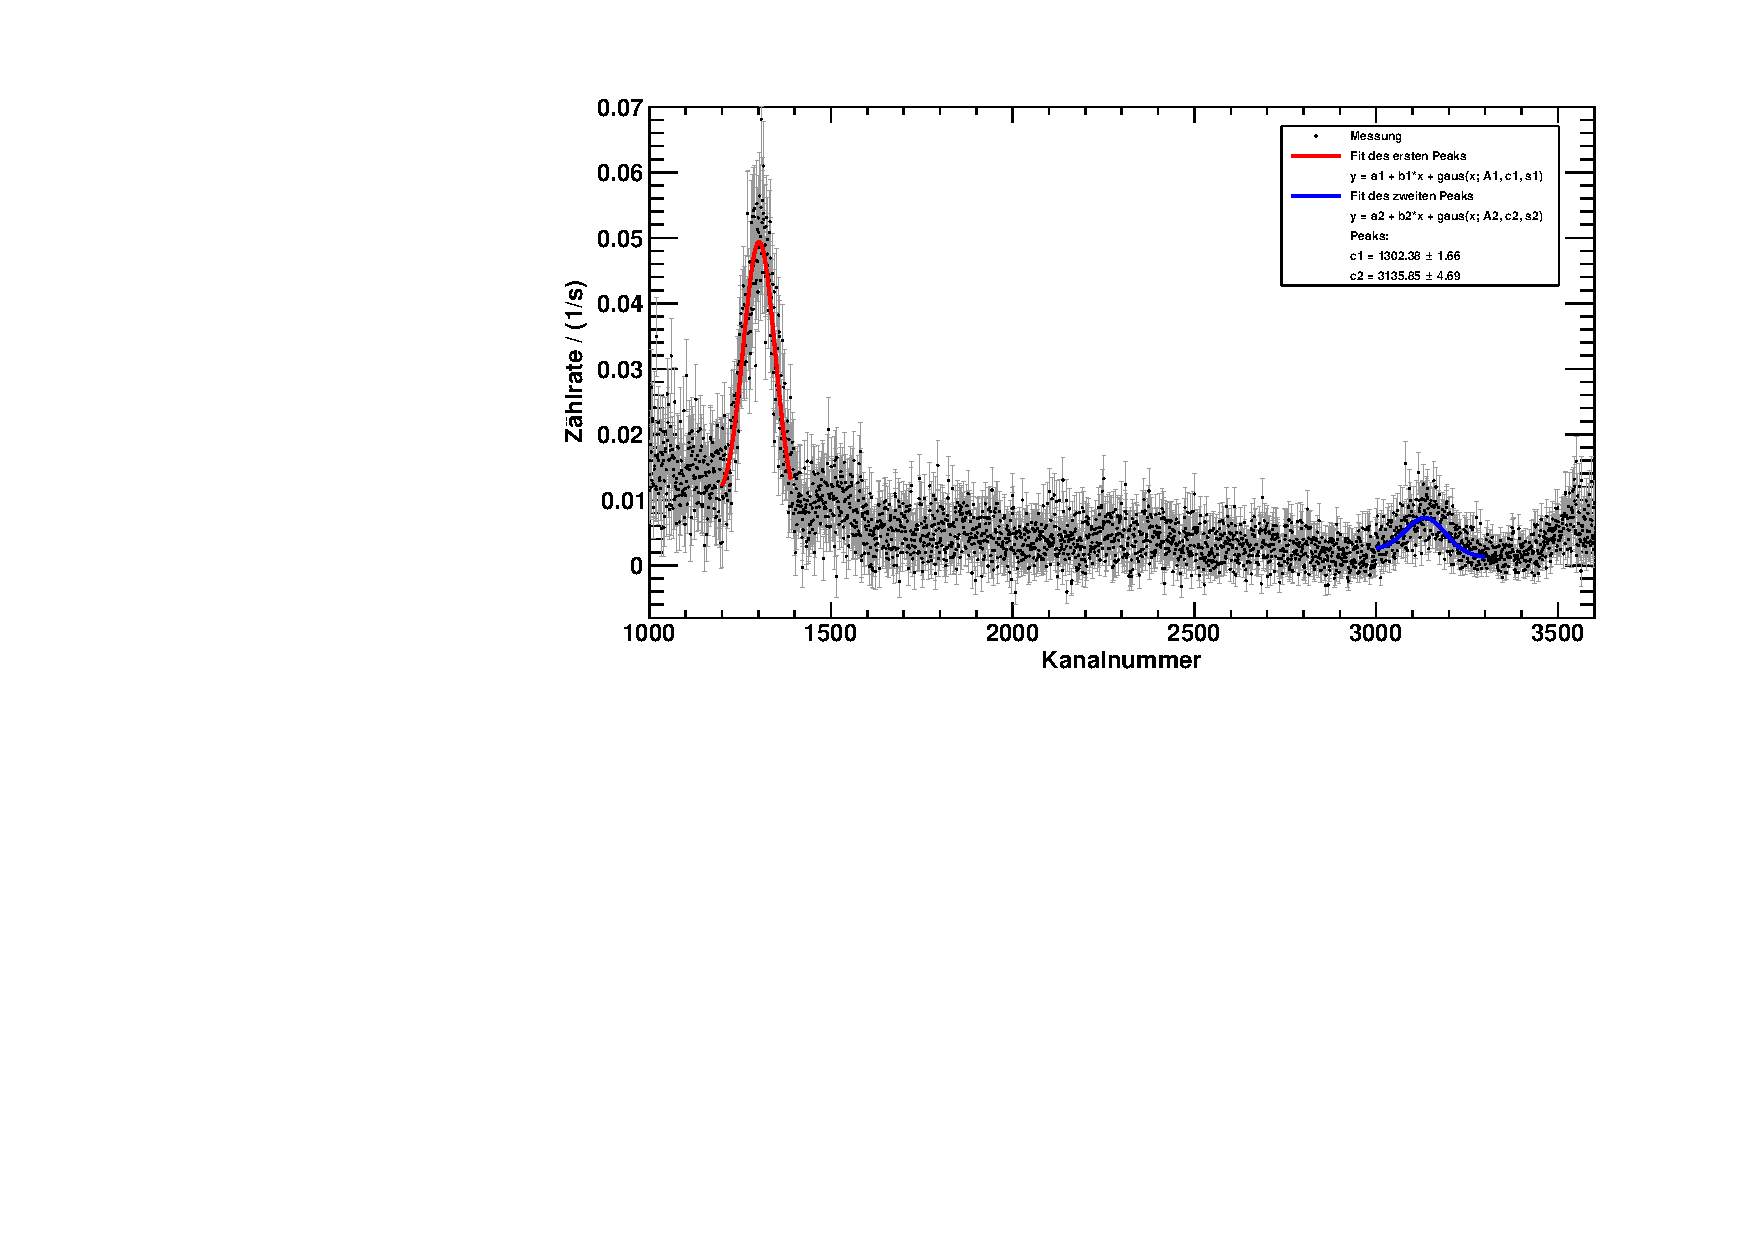
\includegraphics[width=\textwidth]{../img/na_peaks.pdf}
  \caption{\textgamma-Spektrum von \chemel{Na}{22} mit 511\,keV Peak}
  \label{img:na:peak}
\end{center}
\end{figure}

\begin{figure}[H]
\begin{center}
  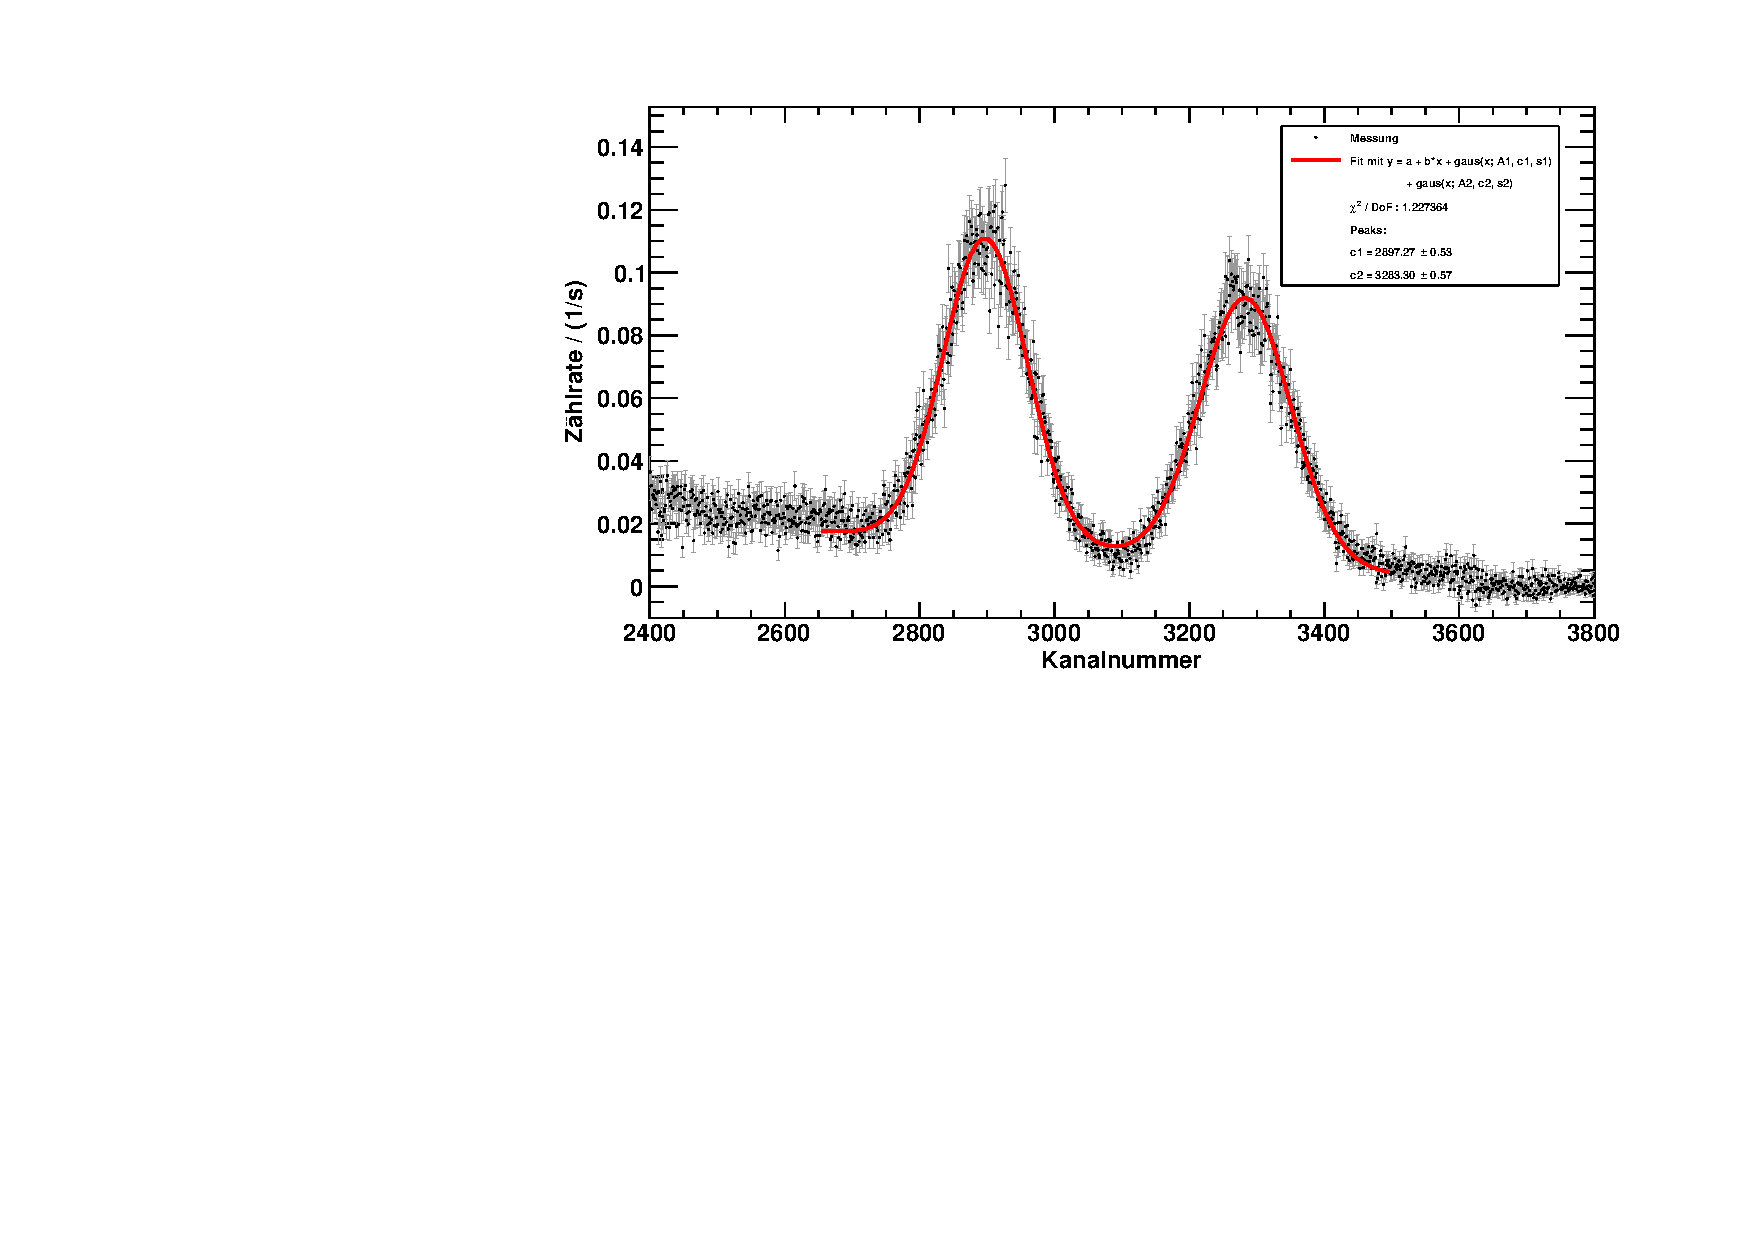
\includegraphics[width=\textwidth]{../img/co_peaks.pdf}
  \caption{\textgamma-Spektrum von \chemel{Co}{60}}
  \label{img:co:peak}
\end{center}
\end{figure}

\begin{figure}[H]
\begin{center}
  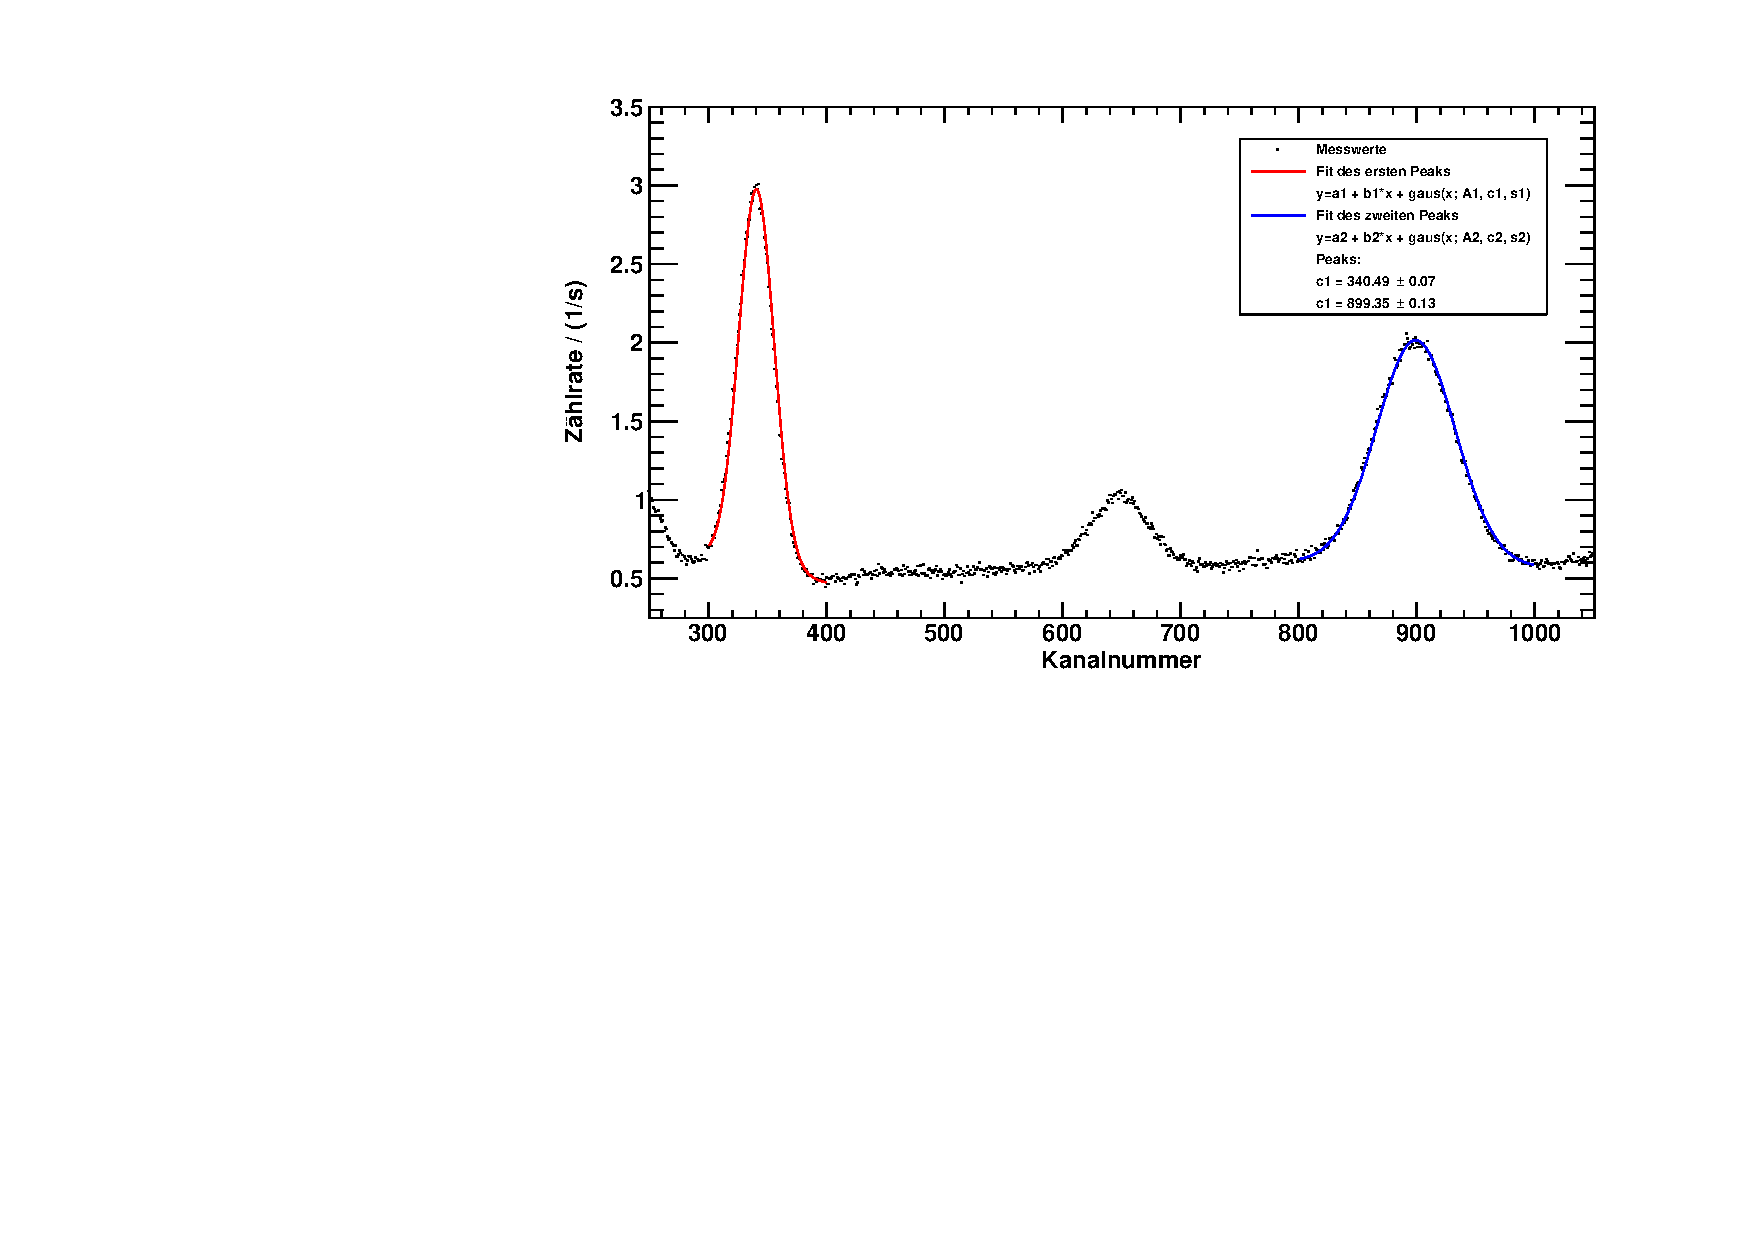
\includegraphics[width=\textwidth]{../img/eu_peaks.pdf}
  \caption{\textgamma-spektrum von \chemel{Eu}{152}}
  \label{img:eu:peak}
\end{center}
\end{figure}

\begin{figure}[H]
\begin{center}
  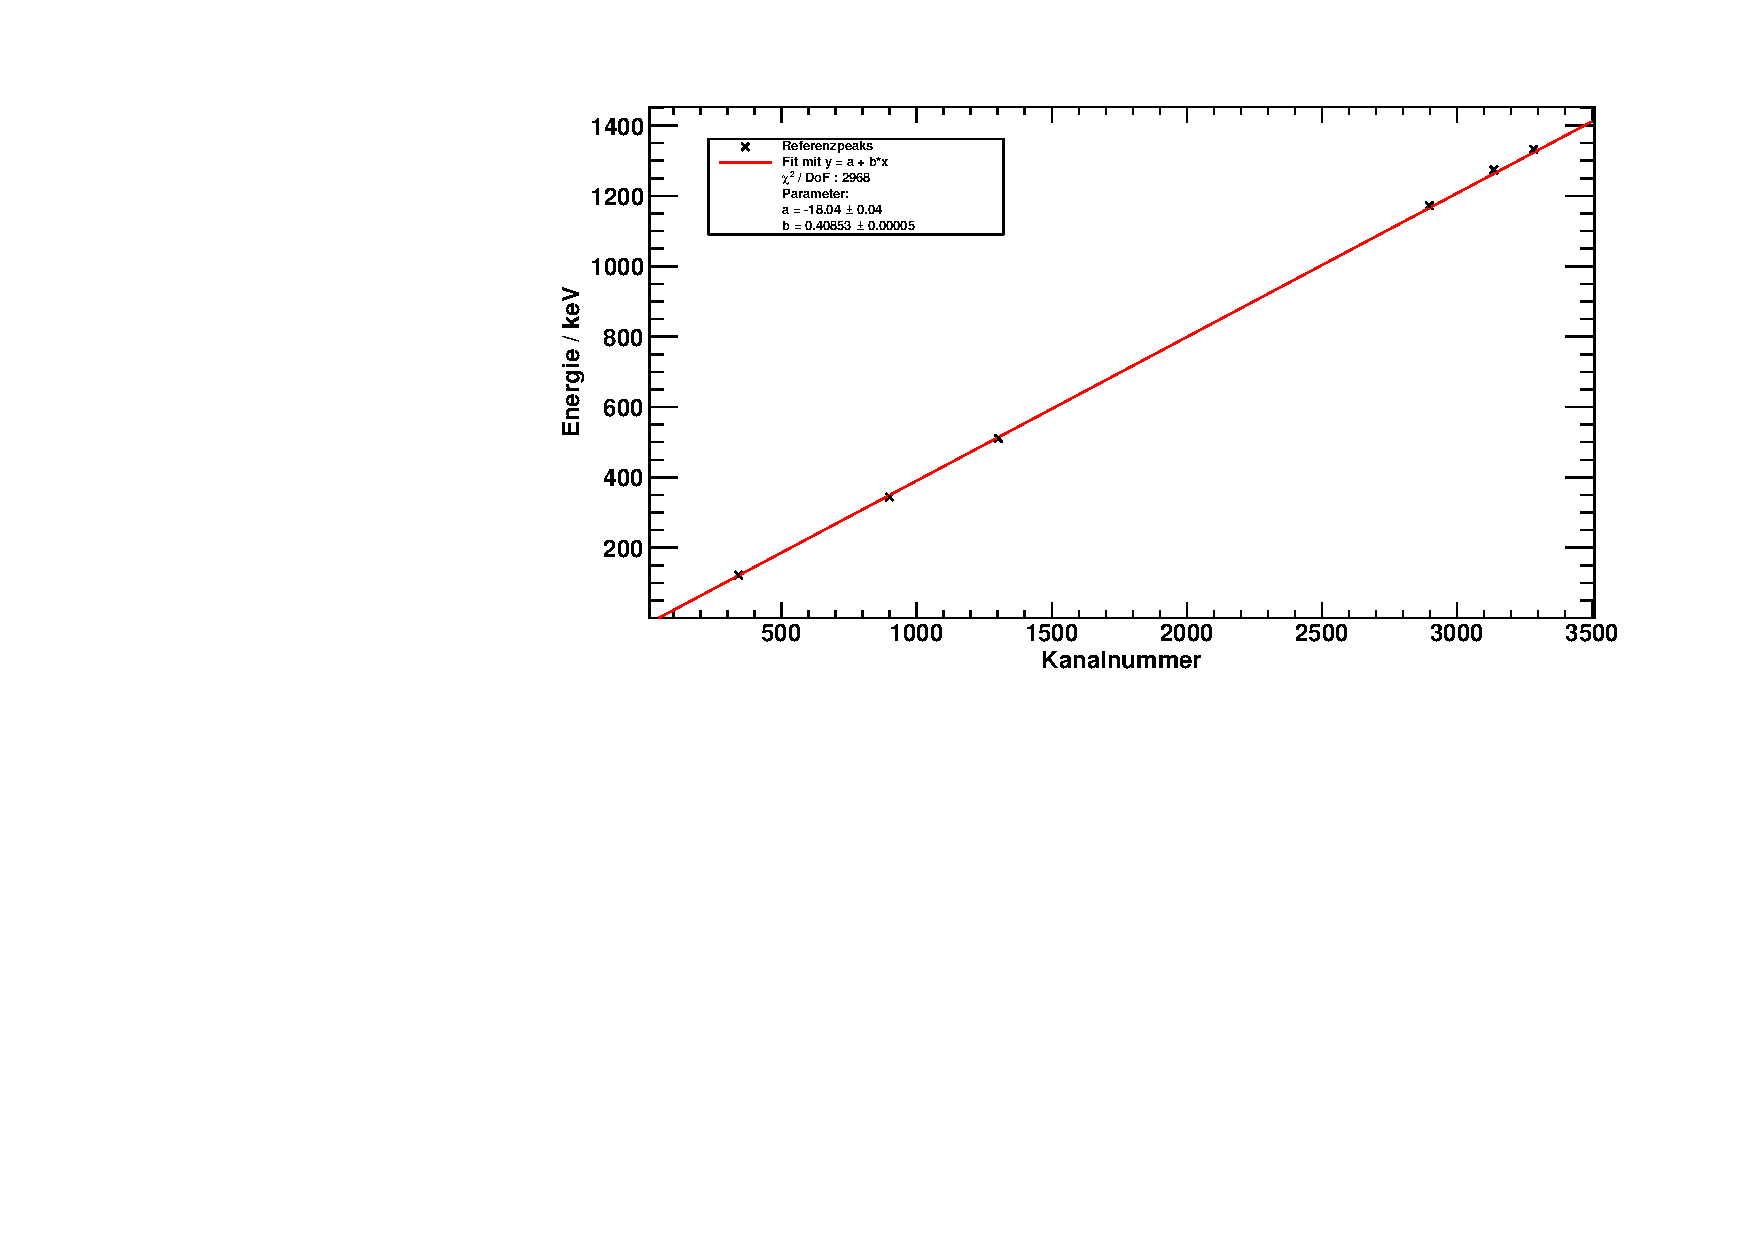
\includegraphics[width=\textwidth]{../img/energy_gauge_lin.pdf}
  \caption{Lineare Energieeichung}
  \label{img:gauge:lin}
\end{center}
\end{figure}

\begin{figure}[H]
\begin{center}
  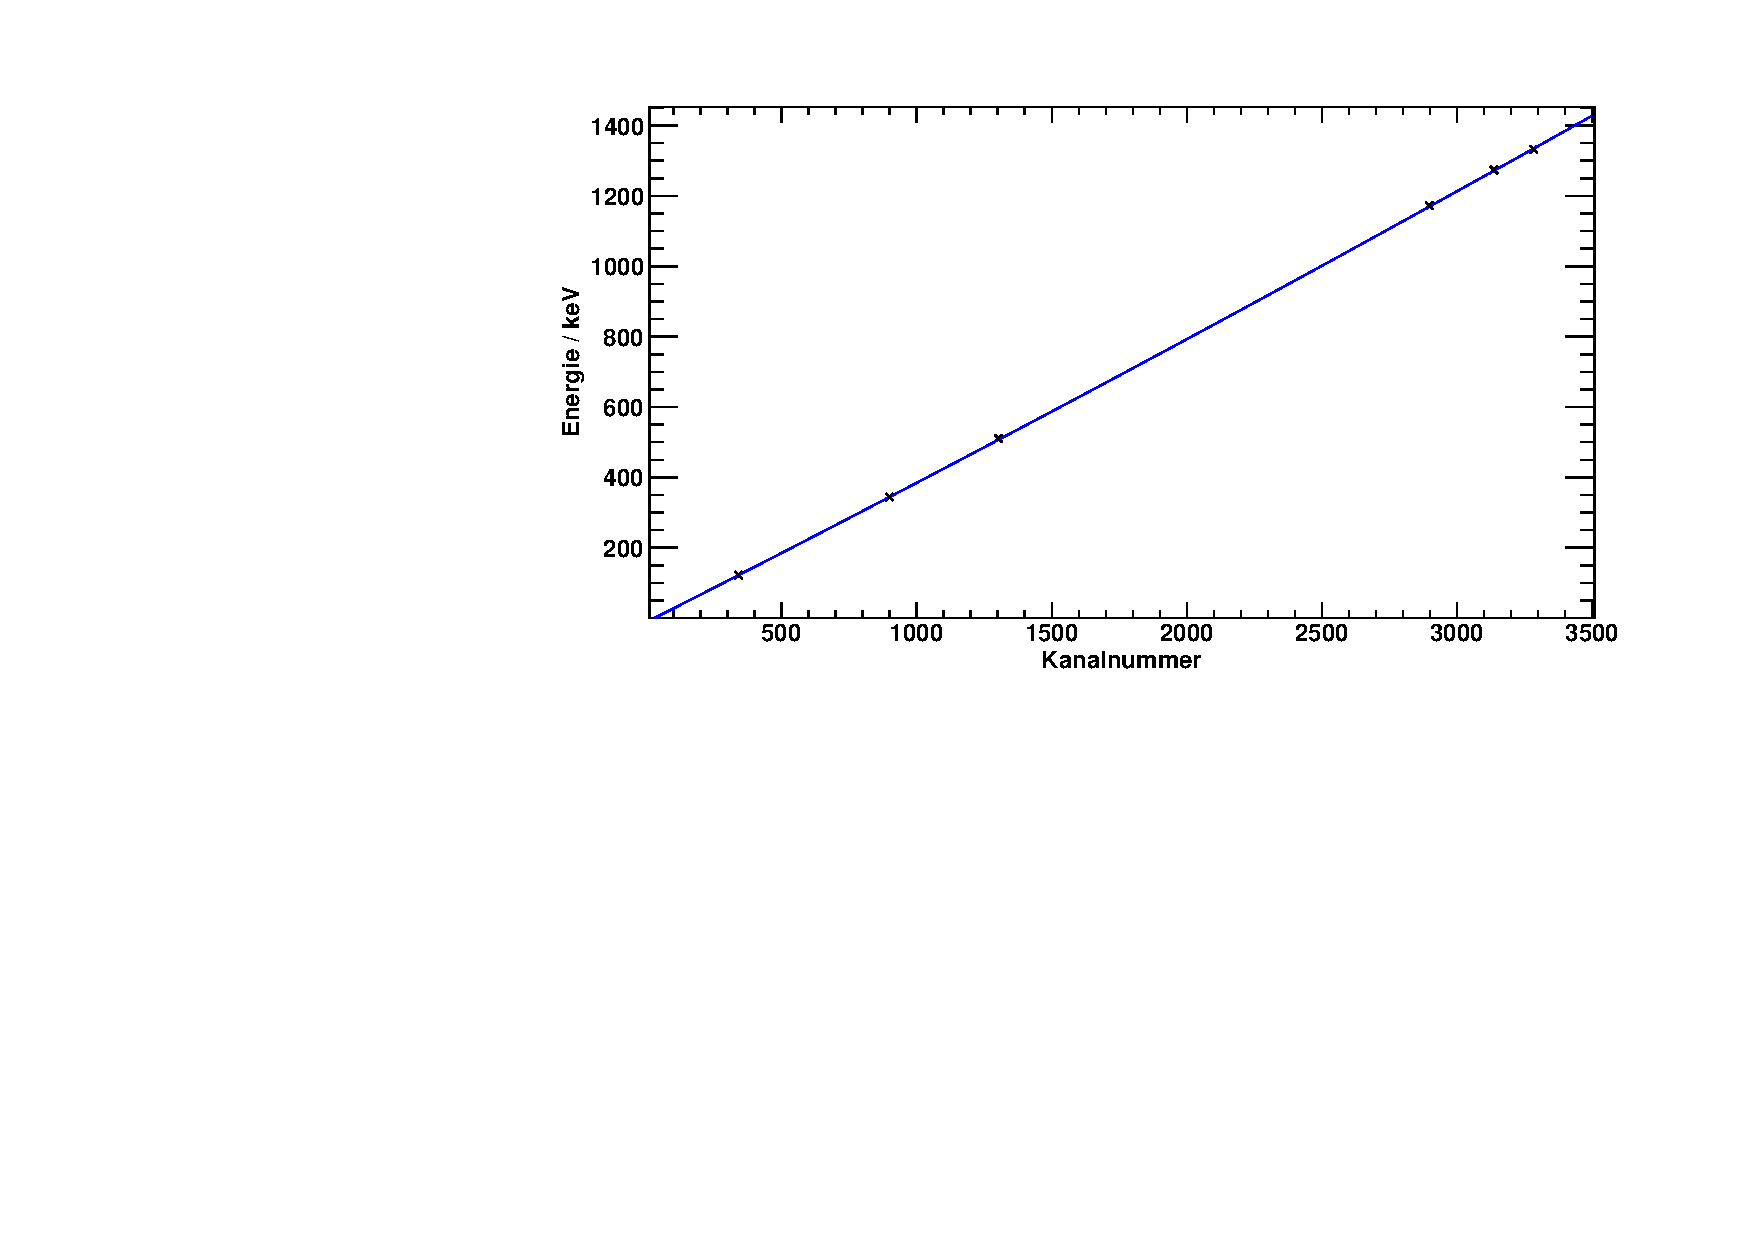
\includegraphics[width=\textwidth]{../img/energy_gauge_quad.pdf}
  \caption{Quadratische Energieeichung}
  \label{img:gauge:lin}
\end{center}
\end{figure}

\subsection{\textgamma-Spektrum von \chemel{Th}{228}}
\begin{figure}[H]
\begin{center}
  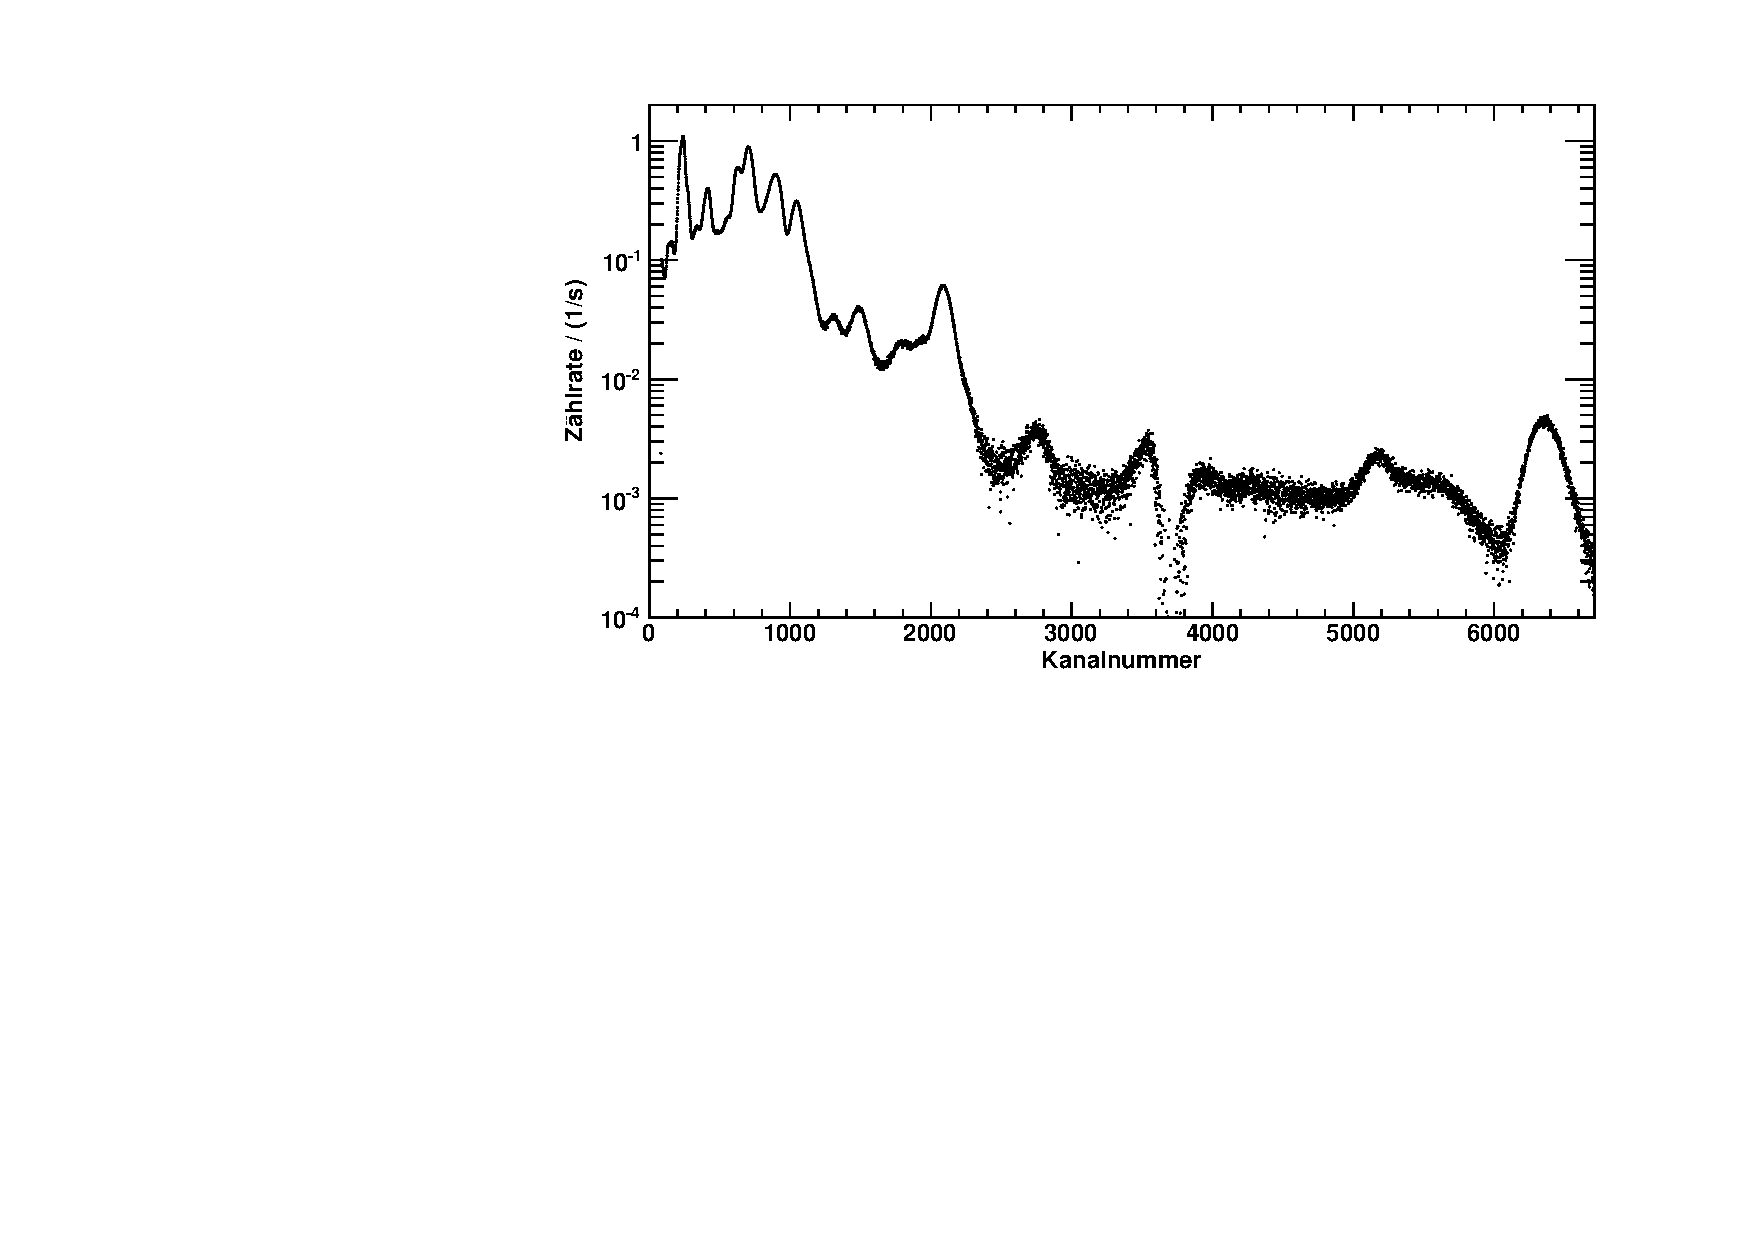
\includegraphics[width=\textwidth]{../img/th_energyspectrum.pdf}
  \caption{\textgamma-Spektrum von \chemel{Th}{228}}
  \label{img:th:spectrum}
\end{center}
\end{figure}

\subsubsection{Single-Peak Fit} % TODO Benennung
\begin{figure}[H]
\begin{center}
  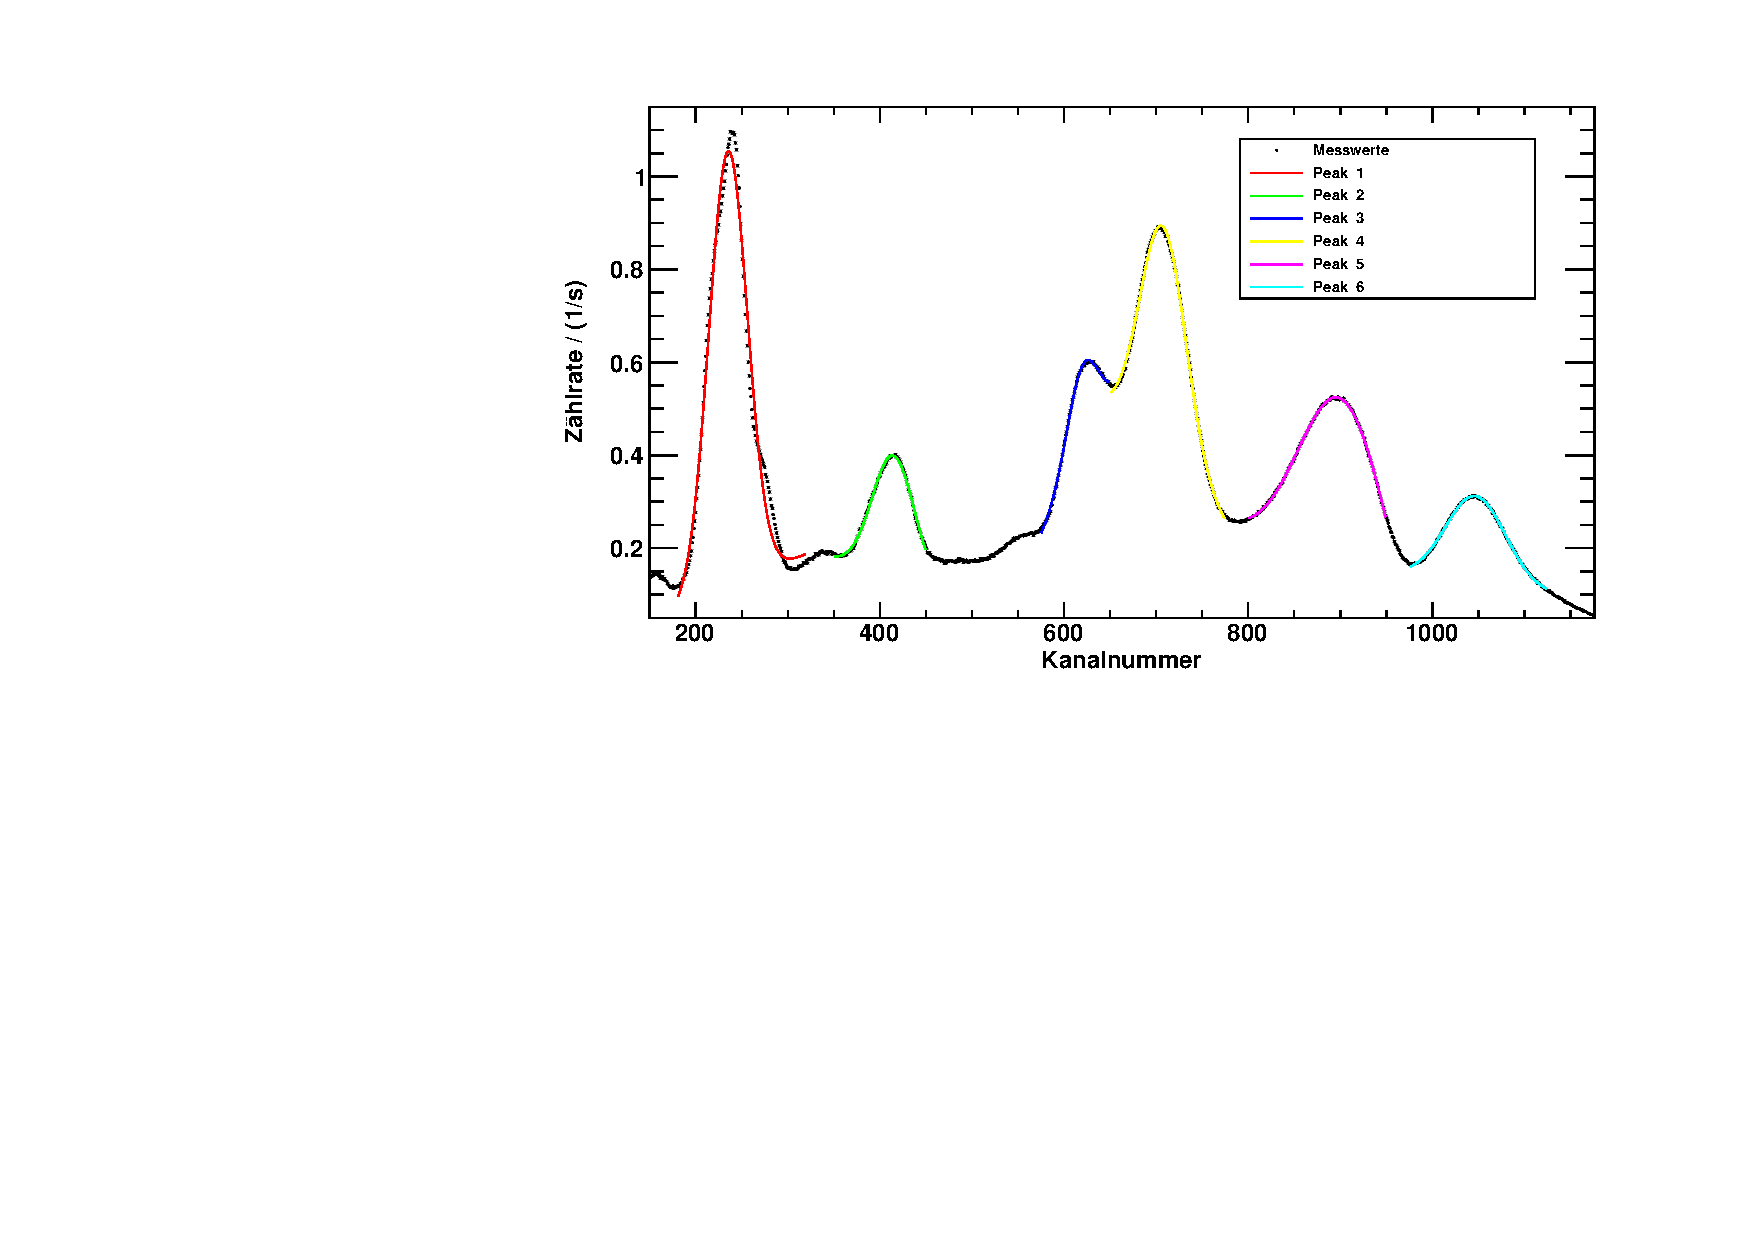
\includegraphics[width=\textwidth]{../img/th_peaks_single_01-06.pdf}
  \caption{Peaks 1 bis 6}
  \label{img:th:peaks:single:0106}
\end{center}
\end{figure}

\begin{figure}[H]
\begin{center}
  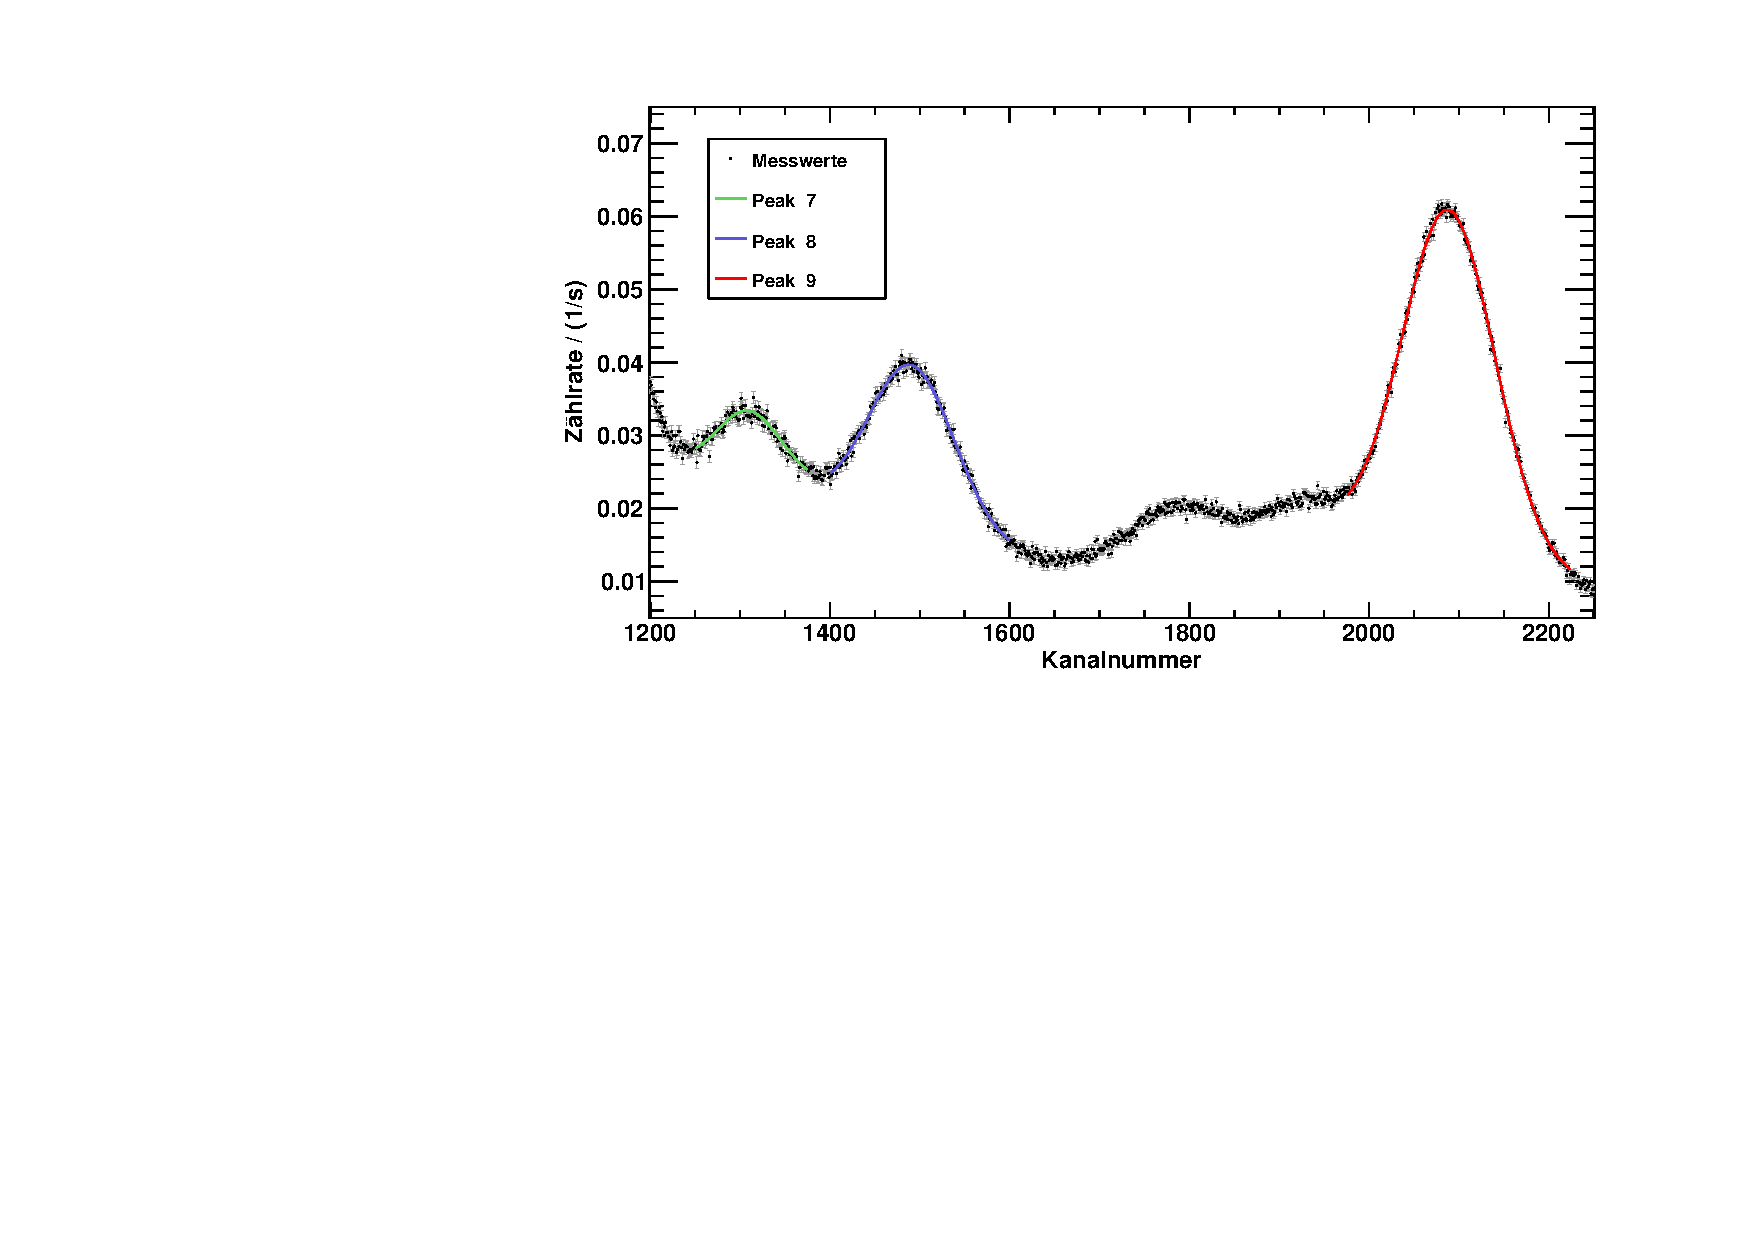
\includegraphics[width=\textwidth]{../img/th_peaks_single_07-09.pdf}
  \caption{Peaks 7 bis 9}
  \label{img:th:peaks:single:0709}
\end{center}
\end{figure}

\begin{figure}[H]
\begin{center}
  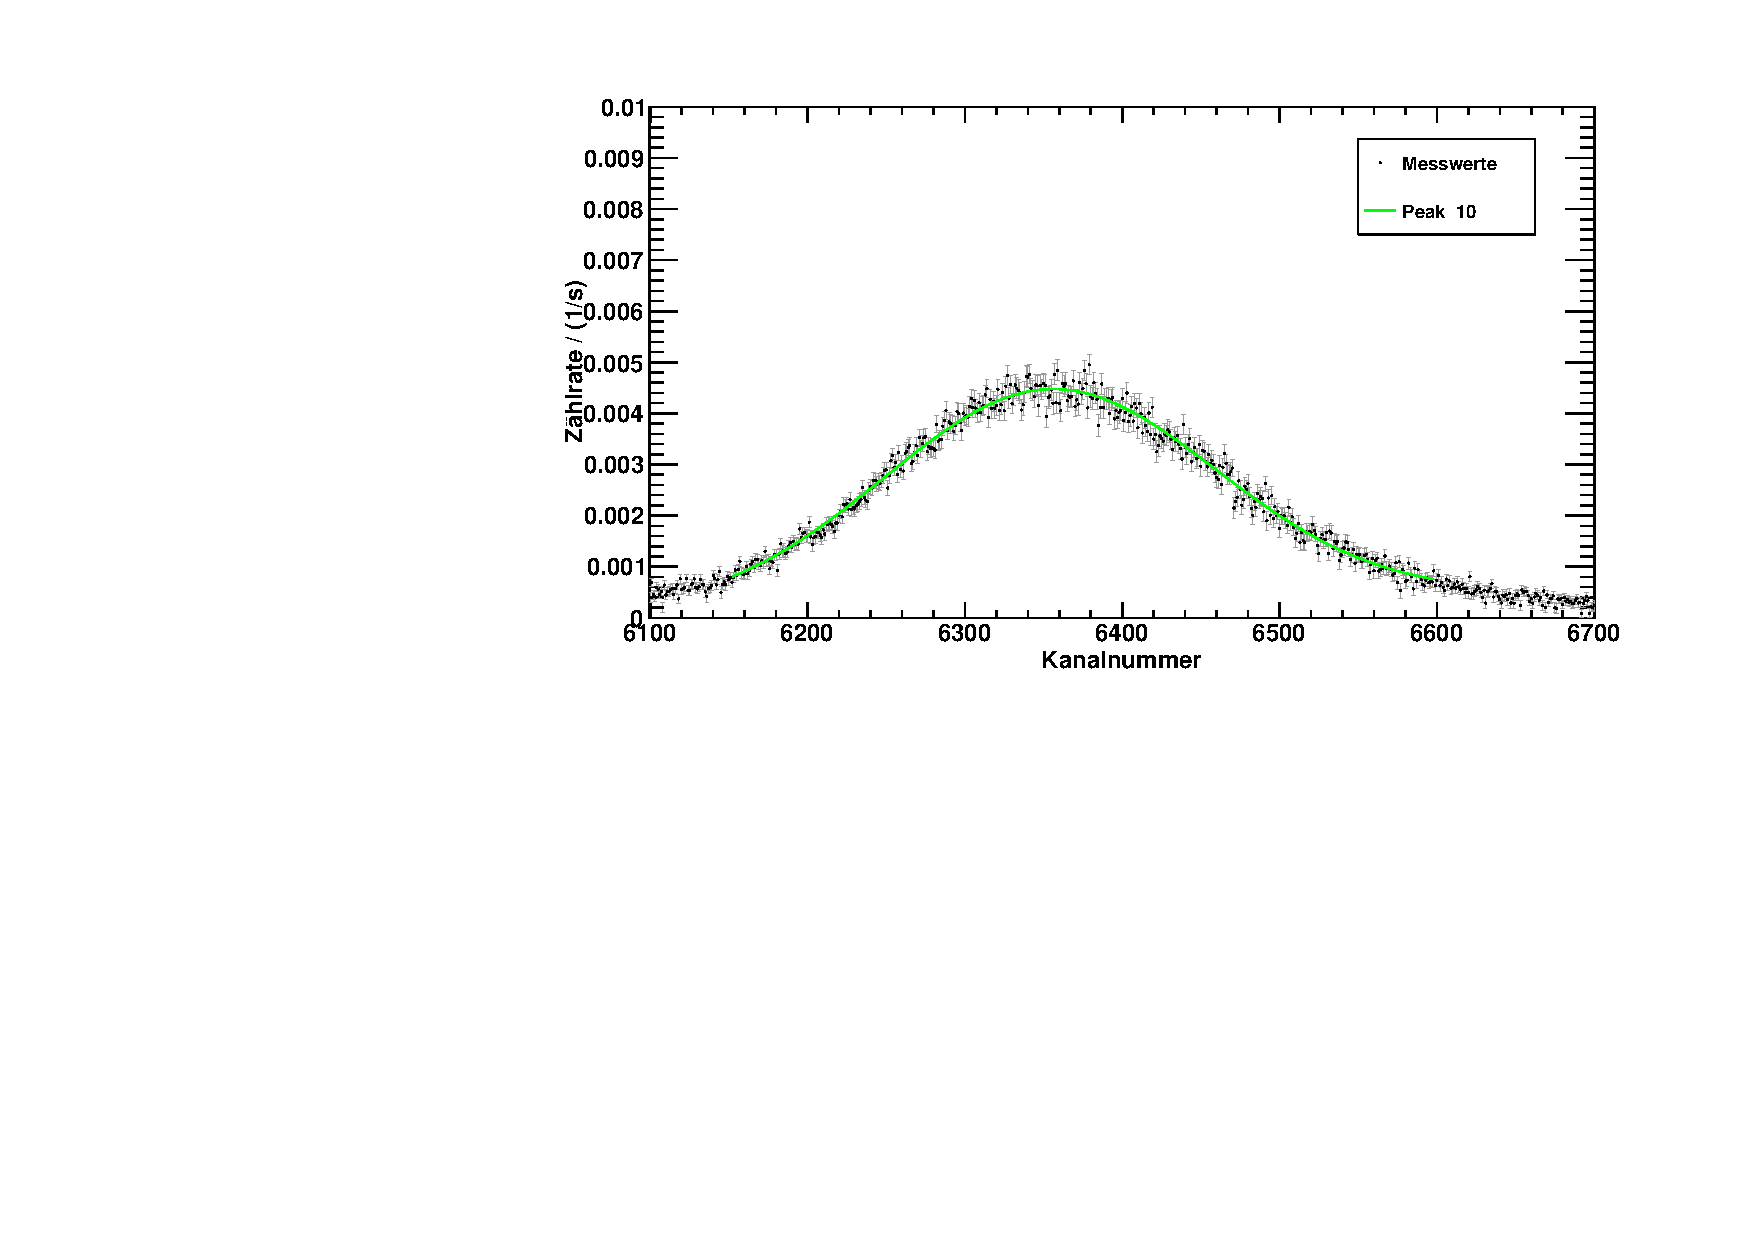
\includegraphics[width=\textwidth]{../img/th_peaks_single_10.pdf}
  \caption{Peak 10}
  \label{img:th:peaks:single:10}
\end{center}
\end{figure}

\subsubsection{Multi-Peak Fit} % TODO Benennung
\begin{figure}[H]
\begin{center}
  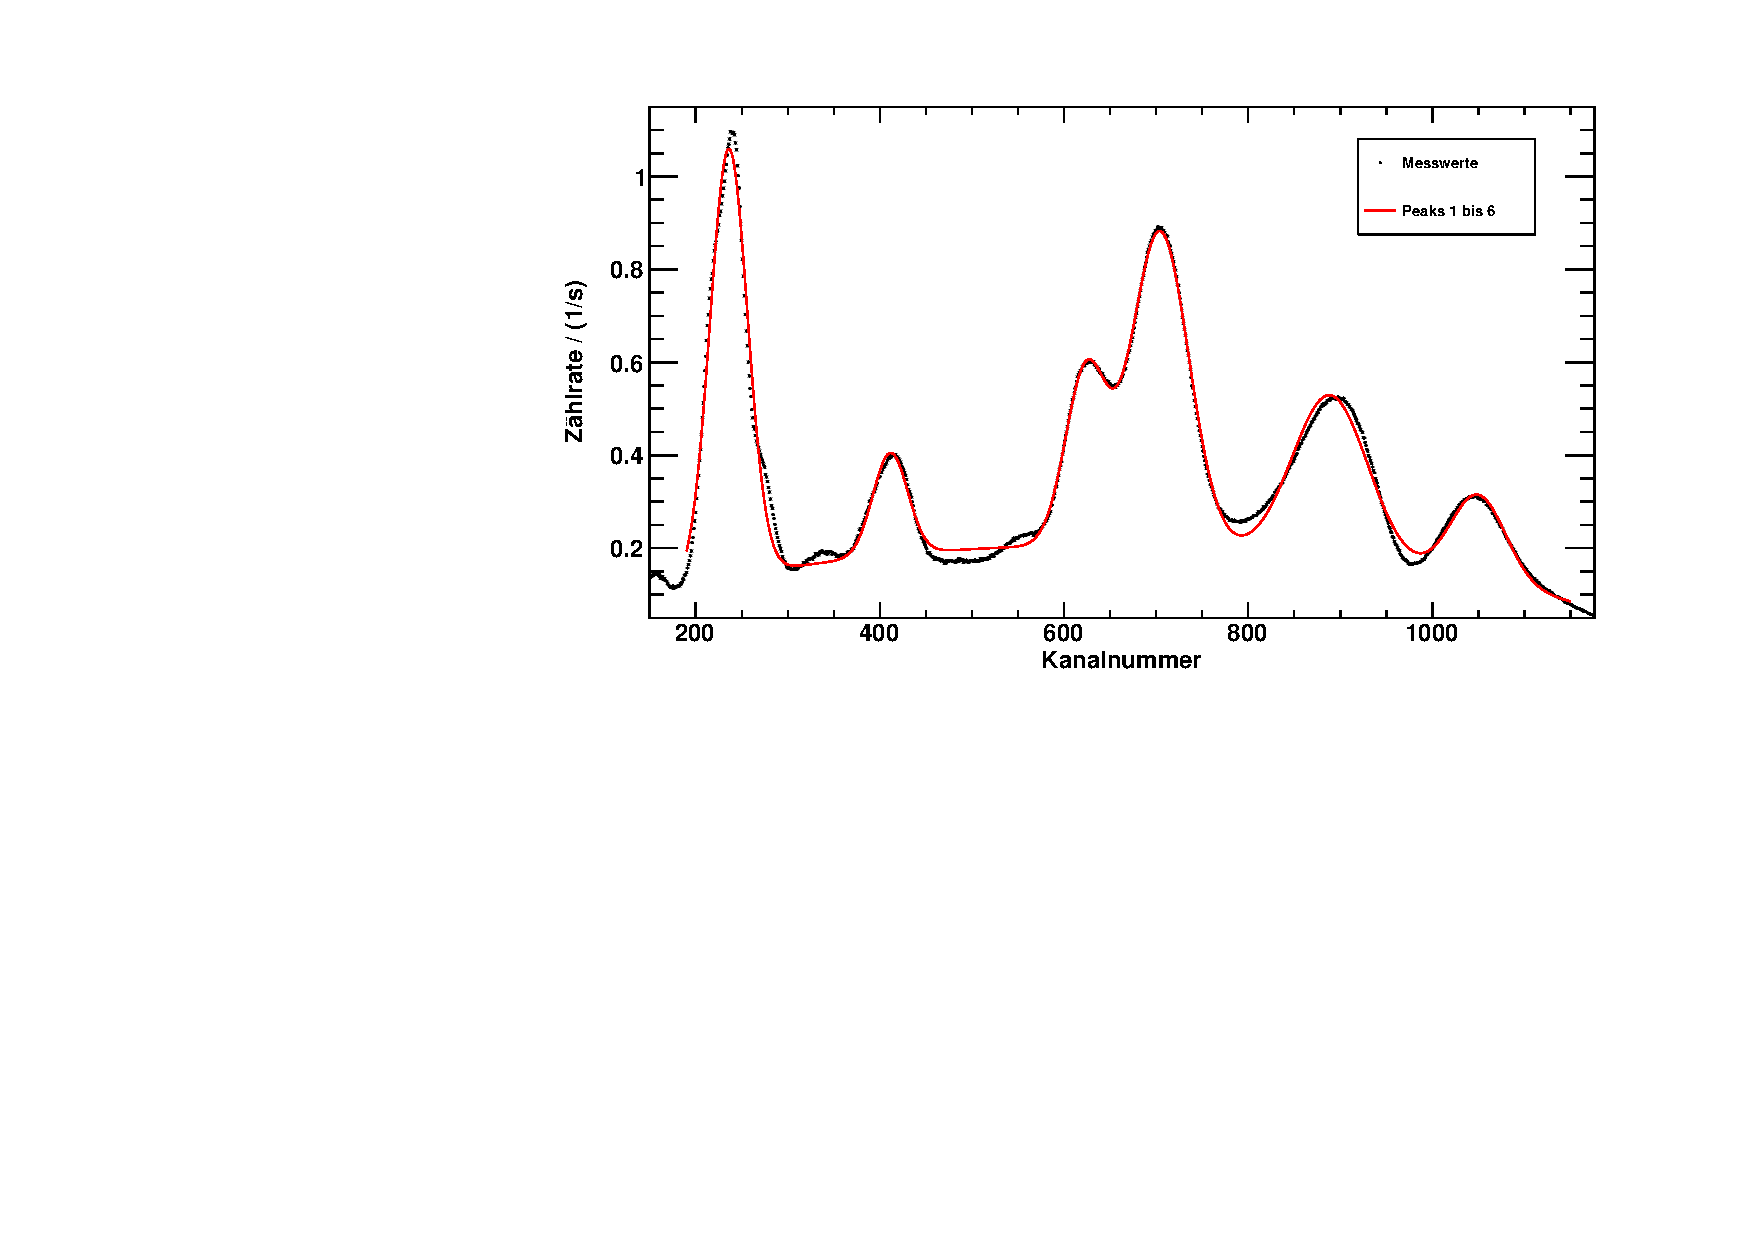
\includegraphics[width=\textwidth]{../img/th_peaks_multi_01-06.pdf}
  \caption{Peaks 1 bis 6}
  \label{img:th:peaks:multi:0106}
\end{center}
\end{figure}

\begin{figure}[H]
\begin{center}
  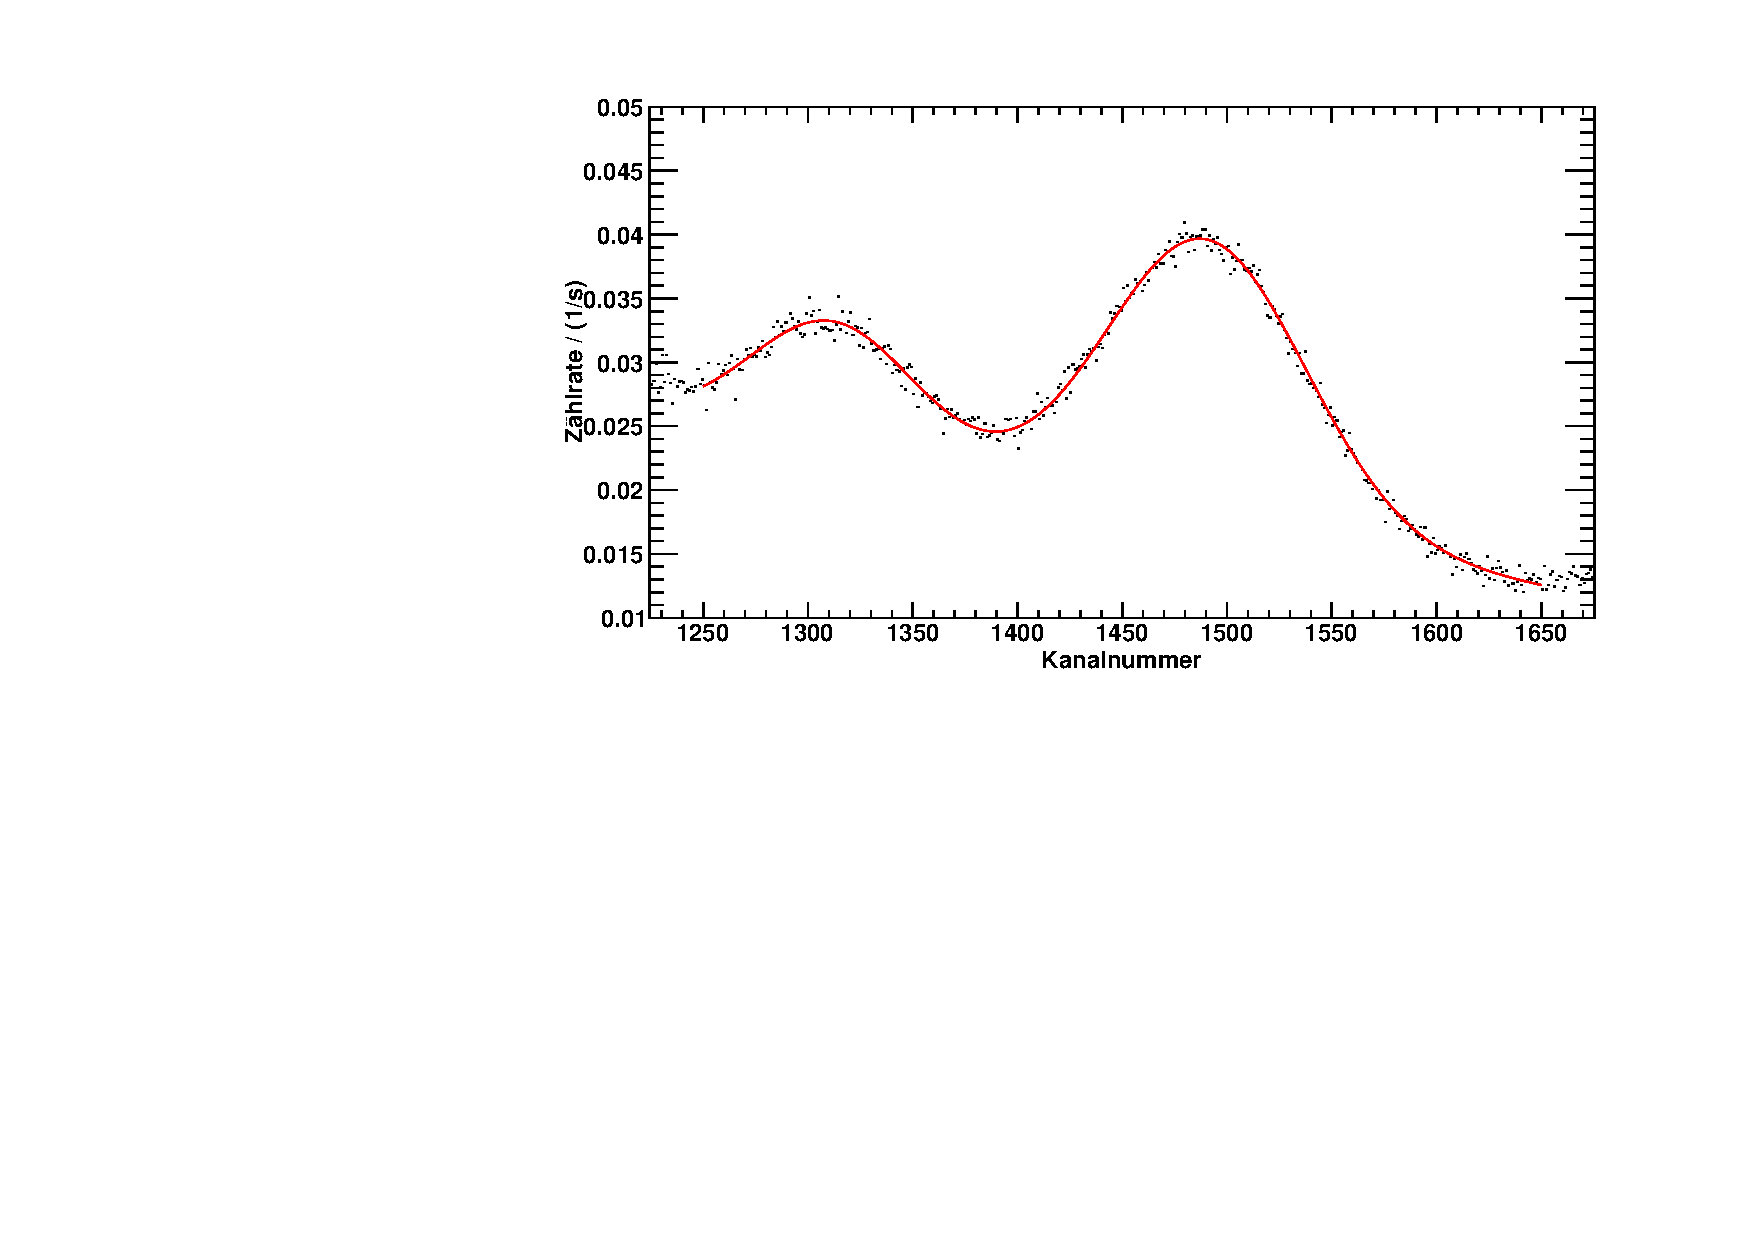
\includegraphics[width=\textwidth]{../img/th_peaks_multi_07-08.pdf}
  \caption{Peaks 7 und 8}
  \label{img:th:peaks:multi:0708}
\end{center}
\end{figure}

\subsection{Untergrund}
\begin{figure}[H]
\begin{center}
  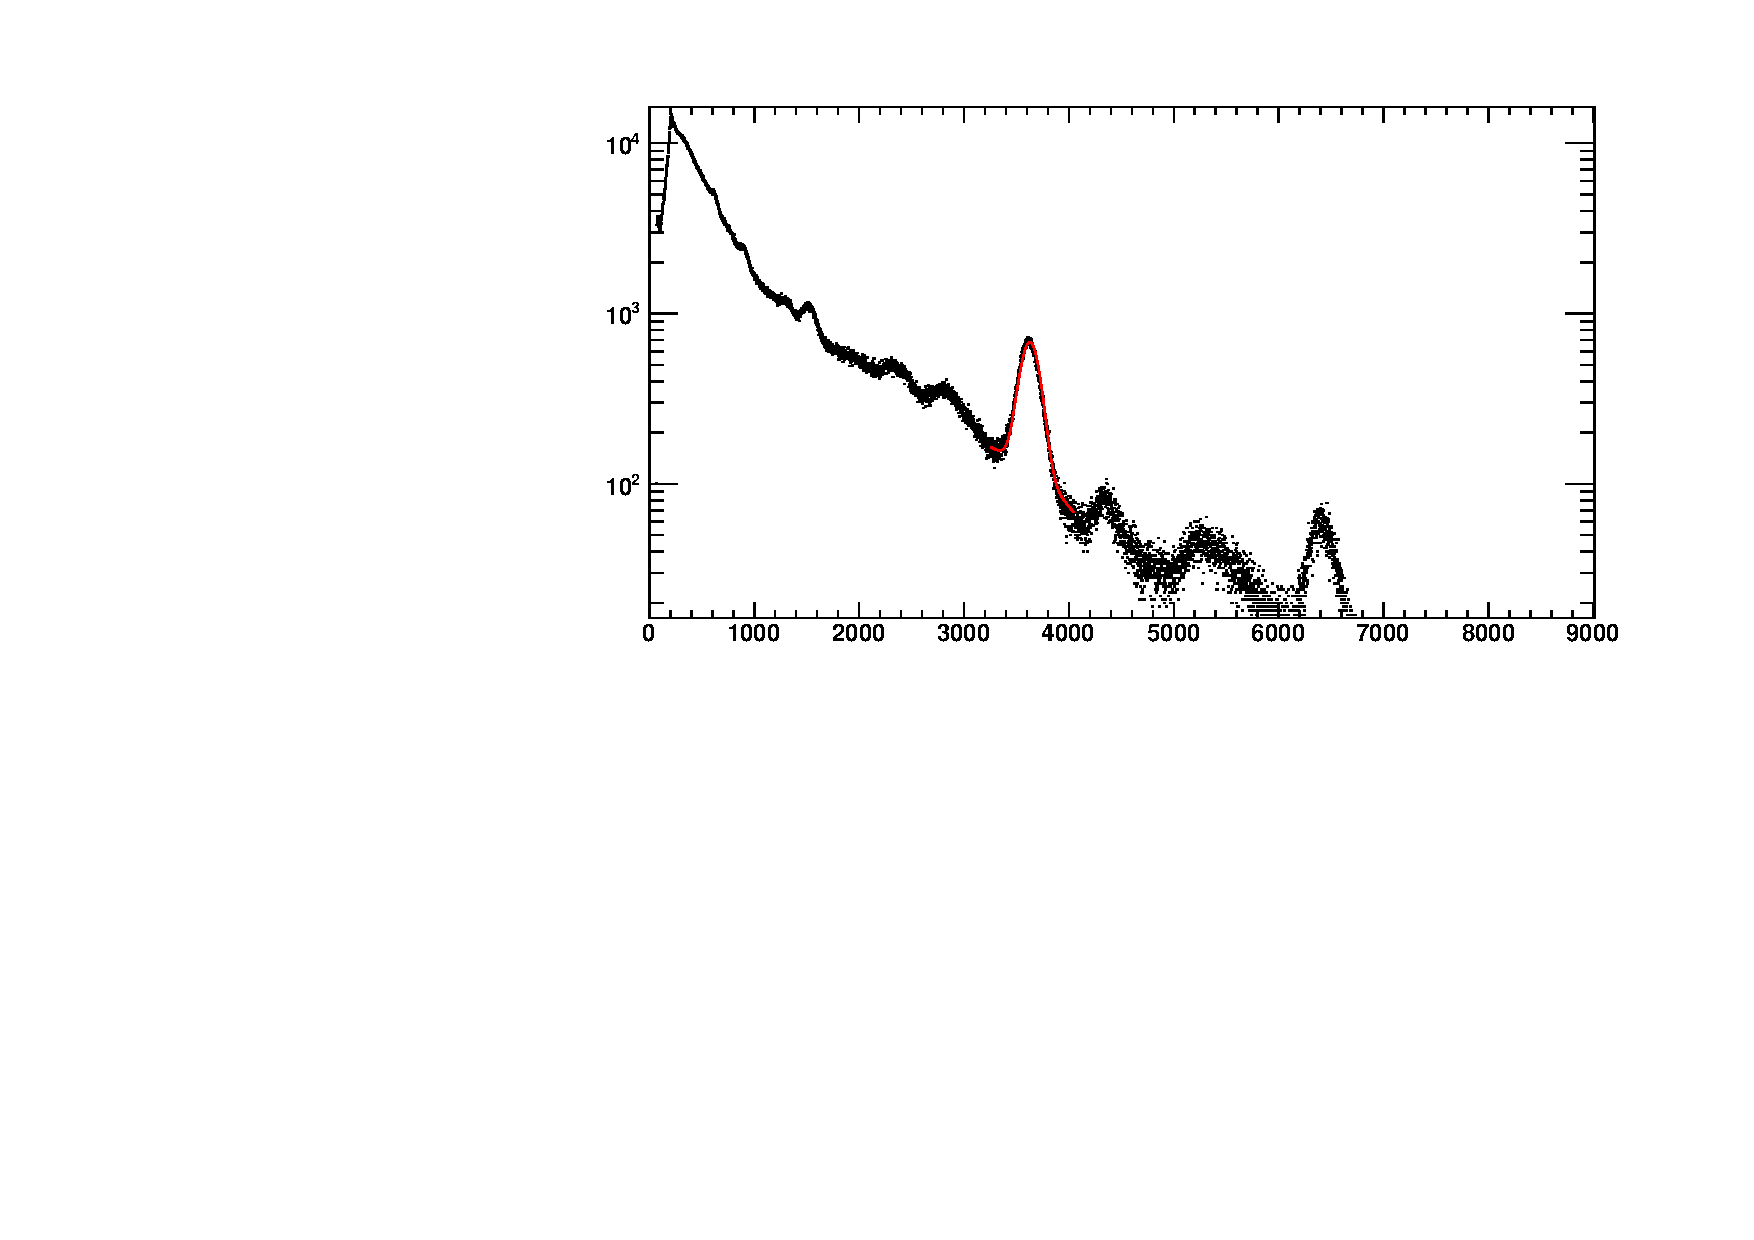
\includegraphics[width=\textwidth]{../img/underground.pdf}
  \caption{Untergrund}
  \label{img:underground}
\end{center}
\end{figure}


\subsection{Winkelkorrelation der \chemel{Na}{22} Vernichtungsphotonen}
\begin{figure}[H]
\begin{center}
  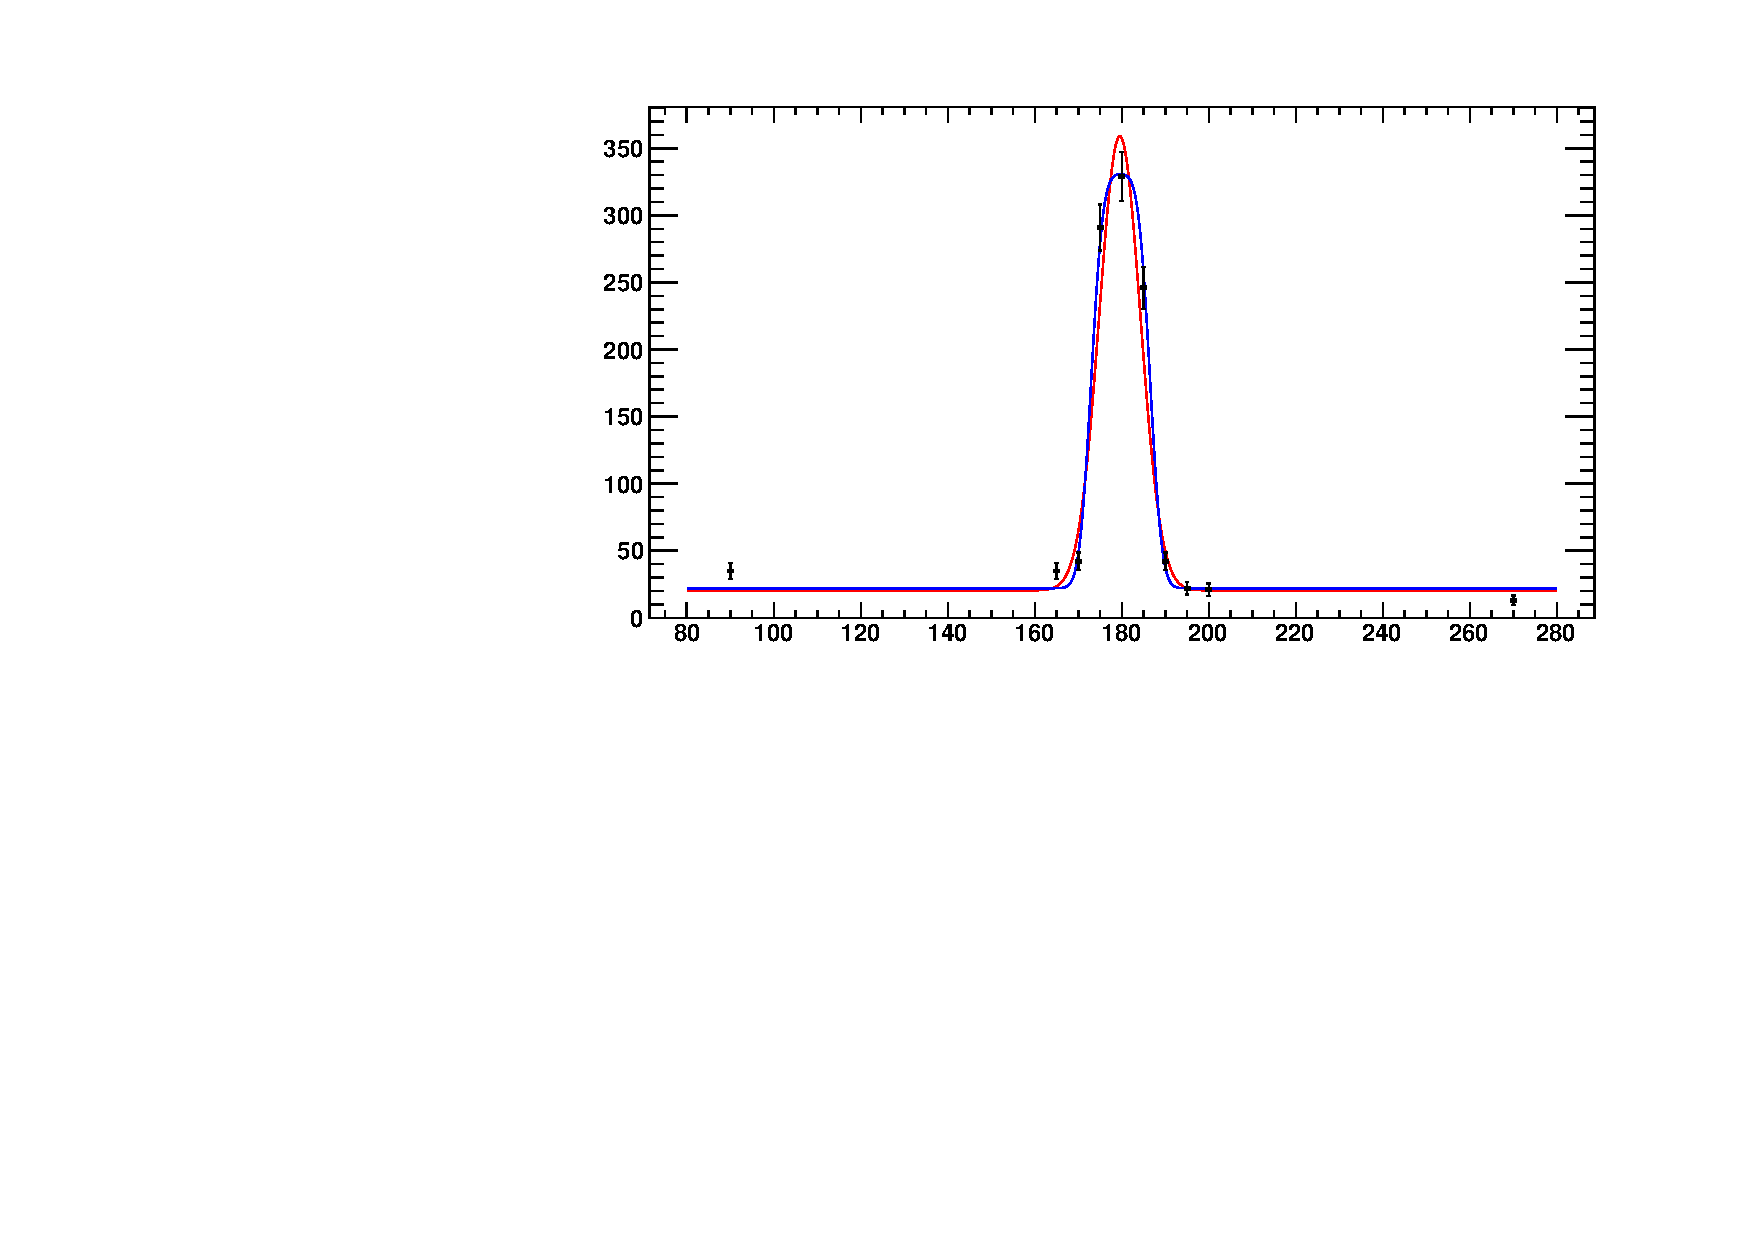
\includegraphics[width=\textwidth]{../img/angles.pdf}
  \caption{Winkelkorrelation der \chemel{Na}{22} Vernichtungsphotonen}
  \label{img:angles}
\end{center}
\end{figure}
